\documentclass[11pt]{article}
% packages
\usepackage[left=1.87cm,right=1.87cm,top=1.87cm,bottom=1.87cm]{geometry}
\usepackage[utf8]{inputenc}
\usepackage{mathrsfs}
\usepackage{multirow}
\usepackage{amsfonts}
\usepackage{amssymb}
\usepackage{amsmath}
\usepackage{float}
\usepackage{mathtools}
\usepackage{amsthm} 
\usepackage{comment}
\usepackage{xcolor}
\usepackage{graphicx}
\usepackage{yhmath}
\usepackage{mathdots}
\usepackage{wasysym}
\usepackage{xargs}
\usepackage[symbol]{footmisc}
\usepackage[shadow,textsize=tiny,tickmarkheight=4pt]{todonotes}

% HURL
\usepackage{hyperref}
\hypersetup{
    colorlinks=true,
    linkcolor=red,
    filecolor=red,      
    urlcolor=red,
    citecolor=red
}
\urlstyle{same}

% Theorem environments
\theoremstyle{definition}
\newtheorem{theorem}{Theorem}
\newtheorem{claim}{Claim}
\newtheorem{proposition}{Proposition}
\newtheorem{lemma}{Lemma}
\newtheorem{remark}{Remark}
\newtheorem{definition}{Definition}

% Math commands
\newcommand{\F}{\mathbb{F}}
\newcommand{\N}{\mathbb{N}}
\newcommand{\C}{\mathbb{C}}
\newcommand{\R}{\mathbb{R}}
\renewcommand{\P}{\mathbb{P}}
\newcommand{\Fp}{\mathbb{F}_p}
\newcommand{\Fpp}{\mathbb{F}_{p^2}}
\newcommand{\vp}{\varphi}
\newcommand{\ra}{\rightarrow}
\newcommand{\vph}{\hat{\varphi}}
\newcommand{\Z}{\mathbb{Z}}

% Keywords command
\providecommand{\keywords}[1]
{
  \smallskip\noindent\small	
  \textbf{\textbf{Keywords---}} #1
}
\newcommand{\LC}[2]{\ensuremath{L_{[#1 : #2]}}}
\newcommand{\Mont}[2]{\ensuremath{M_{#1, #2}}}
\newcommand{\Id}{\mathcal{O}}

% other shortcuts 
\newcommand\mytodo[1]{(\textcolor{red}{{\bf todo}}: #1)}
\def\td{(\textcolor{red}{{\bf todo}})}
\newcommand\done[1]{- \textcolor{red}{{\bf done}} #1}
\def\done{(\textcolor{red}{{\bf done}})}
\def\td{(\textcolor{red}{{\bf todo}}) }
\def\why{(\textcolor{red}{{\bf why?}}) }
\renewcommand{\thefootnote}{\fnsymbol{footnote}}
\DeclarePairedDelimiter{\ceil}{\lceil}{\rceil}
\DeclarePairedDelimiter{\floor}{\lfloor}{\rfloor}
\DeclareMathOperator{\cswap}{cswap}
\DeclareMathOperator{\End}{End}
\DeclareMathOperator{\chr}{char}
\DeclareMathOperator{\bd}{bd}
\DeclareMathOperator{\crit}{crit}


% Algorithms
\usepackage[vlined,ruled,linesnumbered,titlenotnumbered]{algorithm2e}
%\usepackage{algorithm2e}
\newcommand{\Input}{\item[\textsc{Input:}]}
\newcommand{\Output}{\item[\textsc{Output:}]}
\newcommand{\Remark}{\item[\textsc{Remark:}]}
\newcommand{\pushline}{\Indp}% Indent
\newcommand{\popline}{\Indm\dosemic}% Undent
\let\oldnl\nl% Store \nl in \oldnl
\newcommand{\nonl}{\renewcommand{\nl}{\let\nl\oldnl}}% Remove line number for one line
\makeatother


% Tikz
\usepackage{tikz}
\usetikzlibrary{arrows.meta}




\title{A deterministic algorithm for computing one point in each connected component of a smooth real algebraic set}
\author{Jesse Elliott\thanks{David R. Cheriton School of Computer Science, University of Waterloo, On, Canada}, Mohab Safey El Din\thanks{Sorbonne Universit\'e, CNRS, INRIA, Laboratoire d’Informatique de Paris 6, PolSys, Paris, France}, \'Eric Schost \thanks{David R. Cheriton School of Computer Science, University of Waterloo, On, Canada} 
}


\date{}

\def\ms#1{\textcolor{olive}{#1}}
\begin{document}

\maketitle




\begin{abstract}
This is an abstract \newline
\keywords{Real algebraic geometry, polynomial system solving, complexity}
\end{abstract}


\newpage 




%%%%%%%%%%%%%%%%%%%%%%%%%%%%%%%%%%%%%%%%%%%%%%%%%%%%%%%%%%%%%%%%%%%%%%%
\section{Removing the Noether position requirement}
For $i$ in
$\{1,\dots,n\},$ consider the projections
\begin{align*}
    \vp_i: \C^n  &\rightarrow \C^i \\
    (x_1,\hdots,x_n) &\mapsto  (x_1,\hdots,x_i)    
\end{align*}
\begin{align*}
    \psi_i: \C^n  &\rightarrow \C^{n-1} \\
    (x_1,\hdots,x_n) &\mapsto  (x_1,\hdots,x_{i-1},x_{i+1},\hdots,x_n)    
\end{align*}
\begin{align*}
    \pi_i: \C^n  &\rightarrow \C \\
    (x_1,\hdots,x_n) &\mapsto x_i.
\end{align*}
%
\begin{proposition}\label{prop:main}
    Let $V \subset \C^n$ be a smooth affine variety and let $C$ be a connected component of $V \cap \R^n$ with dimension $d$. If, for all $i \in \{1,\hdots,n\}, C \cap \crit(\pi_i,V) = \emptyset$  and  $\pi_i(C) \not = \R$, then there exists distinct $i,j \in\{1,\hdots,n\}$ with
    \[
C \cap \{ x_i= x_j\} \not = \emptyset \textrm{ or }
C \cap \{ x_i= -x_j\} \not = \emptyset. 
    \]
\end{proposition}
%
\begin{lemma}
    There exists $i \in \{1,\hdots,n\}$ with $\pi_i(C)$ not bounded. WLOG assume $i=1.$
\end{lemma}
\begin{proof}
    \td
\end{proof}









































%%%%%%%%%%%%%%%%%%%%%%%%%%%%%%%%%%%%%%%%%%%%%%%%%%%%%%%%%%%%%%%%%%%%%%
\subsection*{Assume the dimension of $C$ is $1$}
%
%
\begin{figure}[!h]
    \centering
    

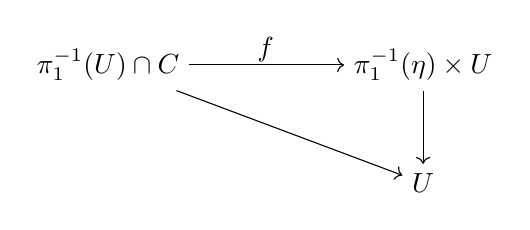
\begin{tikzpicture}

%%    NODES   %%
\node (20) at (-4,3) {$\pi_1^{-1}(U) \cap C$};
\node (21) at (0,3) {$\pi_1^{-1}(\eta) \times U$};
\node (100) at (0,1.5) {$U$};
\node (Order2) at (-2,3.2) {$f$};

%%    ARROWS    %%
\draw [->] (20) -- (100);
\draw [->] (21) -- (100);
\draw [->] (20) -- (21);

\end{tikzpicture}
    \caption{(Finish diagram \td) A Nash version of Ehresmann's fibration theorem.}
    \label{fig:Ehresmann}
\end{figure}
%
%
\begin{proof}
First notice that, for all $i \in \{1,\hdots,n\},$ since $\crit(\pi_i,C) = \emptyset$ and $\pi_i(C) \not = \R$, $\pi_i(C)$ is an open interval:
\[
\pi_i(C)=
\begin{cases}
			(e_i,+\infty), \\
                (-\infty,e_i),\textrm{ or }\\
                (e_i,e_i').
\end{cases}
\]
Now let $U$ denote $(e_1,+\infty)$ and take $\eta \in U.$ A Nash version of
Ehresmann's fibration theorem \cite[Th. 2.4 and 3.1]{Shiota1992} can be given in
terms of Nash functions, $\C^{\infty}$\todo{change notation $\mathcal{C}^\infty$} semi-algebraic functions (see Figure \ref{fig:Ehresmann} for a visual representation). As a consequence of applying the theorem, we obtain a parameterization of $C$ in terms of semi-algebraic functions
\[
\big\{\vartheta(t) = (t,g_2(t),\hdots,g_n(t))~|~ t \in U\big\} \subset C
\]
The semi-algebraic functions $g_2(t),\hdots,g_n(t)$ are diffeomorphisms, and the
tangent vector \ms{at $C$ to $\vartheta(t)$} is given by 
\[
\begin{pmatrix}
    1 \\
    g'_2(t)\\
    \vdots\\
    g'_n(t)\\
\end{pmatrix}.
\]
The tangent vector at a critical point\todo{Not so clear; I believe there is a
  mistake. Only one partial derivative cancels.} would give
\[
\begin{pmatrix}
    1 \\
    g'_2(t)\\
    \vdots\\
    g'_n(t)\\
\end{pmatrix}
=
\begin{pmatrix}
    1 \\
    0\\
    \vdots\\
    0\\
\end{pmatrix}.
\]
Since by assumption, 
\[
C \cap \crit(\pi_i,V) = \emptyset, \forall i \in \{1,\hdots,n\},
\]
$g_2',\hdots,g_n'$ never vanish and therefore $g_2,\hdots,g_n$ are monotonic. Now, consider the set 
\[
N_1 = \big\{i~|~g_i(t) \rightarrow \infty \textrm{ as } t \rightarrow e_1, \textrm{ and } g_i(t) \not \rightarrow \infty \textrm{ as } t \rightarrow \infty\big\},
\]
and notice that when $N_1 \not = \emptyset$ then $x_1 \pm x_i=0$ meets the
connected component $C$\todo{We should make this super precise I guess.},
proving Proposition \ref{prop:main} for the $d=1$ case. And indeed, since
$g_2,\hdots,g_n$ are monotonic, it must be that $N_1$ is not empty.
\color{red}Firstly, there exists an $i$ with $g_i(t) \rightarrow \infty$ as $t
\rightarrow e_1$ because $e_1$ is the boundary point of $\pi_1(C)$ (needs
justification?)\color{black} \ms{Yes. The idea is to say that, if for some $i$
  $\pi_i(\vartheta(t))$ tends to $\infty$ when $t\to 1$, then $i\in N_1$ because
  $g_i$ is monotone (and $\pi_i(C)\neq \R$)}. WLOG assume $i=2.$ Now, since
$g_2(t)$ is monotonic, as $t$ ranges from $e_1$ to $+\infty, g_2(t)$ is
decreasing and thus $g_2(t)$ is monotonically decreasing. We cannot have that
$g_2(t)$ tends to $-\infty$ because then as $t$ tends from $e_1$ to $+\infty$,
$g_2(t)$ would cover the entire real line which we have assumed is not the case.
Therefore, $g_2(t) \rightarrow e_2$ as $t$ tends from $e_1$ to $+\infty$.
\end{proof}
%
%\begin{lemma}
%    \td
%\end{lemma}
%\begin{proof}
%Let $\mathscr{D} = \bd(\vp_2(C))$, let 
%\[
%T_{\epsilon}\mathscr{D} = \left\{\alpha \in \R\langle \epsilon \rangle^2~|~dist(\alpha,\mathscr{D}) \leq \epsilon \right\} 
%\]
%and let $(\zeta_l)_{l \in \N} \subset C$ be a sequence with 
%\[
%\zeta_l \in \pi_1^{-1}\left(e_1 + 1/l \right) \cap \vp_2^{-1}\left(T_{\epsilon}\mathscr{D}\right) \cap C \not = \emptyset~\td.
%\]
%By construction, $\pi_1(\zeta_l) \rightarrow e_1$. Now, 
%\[
%\pi_2(\vp_2(\zeta_l)) \rightarrow ?
%\]
%\td
%\end{proof}
%


%\begin{lemma}
%    Where $d = \dim (C),$ there exists $\{i_1,\hdots,i_d\} \subset \{1,\hdots,n\}$ with $\pi_j(C)$ unbounded for all $j \in \{i_1,\hdots,i_d\}.$
%\end{lemma}


\subsection*{Assume the dimension of $C$ is $d\geq 1$}
\begin{proof}
\td
\end{proof}




\newpage 
\bibliographystyle{plain}
\bibliography{references.bib}
\newpage 







\appendix

\section{Alternative arguments for Proposition \ref{prop:main}}


%
%%%%%%%%%%%%%%%%%%%%%%%%%%%%%%%%%%%%%%%%%%%%%%%%%%%%%%%%%%%%%%%%%%%%%%
\subsection*{Assume the dimension of $C$ is $1$}

%%%%%%%%%%%%%%%%%%%%%%%%%%%%%%%%%%%%%%%%%%%%%%%%%%%%%%%%%%%%%%%%%%%%%%


\subsection*{First argument}
Since $\pi_1(C) \not = \R$ and since $C \not = \emptyset$, there exists 
\[
a \in \bd(\pi_1(C)) = \overline{\pi_1(C)} - \vp_{1}^o(C).
\]
Since $C \cap \crit(\pi_1,V) = \emptyset, a \not \in \pi_1(C).$ Therefore we can take a sequence $(\alpha_l)_{l \in \N} \subset C,$ with $\pi_1(\alpha_l) \rightarrow a$ as $l \rightarrow \pm\infty$; WLOG assume $l \rightarrow +\infty.$ Then, $||\alpha_l|| \rightarrow \infty$ as $l \rightarrow \infty.$ Now, there exists an $i \in \{1,\hdots,n\}$ with $\pi_i(\alpha_l) - \pi_1(\alpha_1) \rightarrow \infty$ as $l \rightarrow \infty.$ 
\par 
Similarly, there exists 
\[
b \in \bd(\pi_i(C)) = \overline{\pi_i(C)} - \pi_i^o(C), b \not \in \pi_i(C).
\]
And therefore a sequence $(\beta_k)_{k \in \N} \subset C$ exists with $\pi_i(\beta_k) \rightarrow b$ and $|| \beta_k|| \rightarrow \infty$ as $k \rightarrow \infty.$ Therefor  $j \in \{1,\hdots,n\}-\{i\}$ exists with 
\[
\pi_j(\beta_k) - \pi_i(\beta_k) \rightarrow \infty
\]
\color{red}
Can we show that 
\[
\pi_1(\beta_k) \rightarrow \infty?
\]
\color{black}
If $n=2$ then since $i \not = 1$, it must be that $i=2$ and $j=1$ so that  $\pi_1(\beta_k) - \pi_2(\beta_k) \rightarrow \infty$ and $\pi_1(\beta_k) \rightarrow \infty.$ And therefore we have a sign change with $x_1-x_2=0$ over the connected component $C$. 
\par 
Let 
\[
N = \big\{i \in \{1,\hdots,n\} ~|~ \psi_i(C) \textrm{ is closed}\big\}. 
\]
\begin{enumerate}
    \item $N = \emptyset:$ 
    \par 
    Since $N$ is empty, $\vp_{n-1}(C)$ is not closed. It follows that $\dim(\vp_{n-1}(C))=1$ because, otherwise, since $C$ is non-empty  and since dimension can only decrease after projection, $\dim(\vp_{n-1}(C))=0$ implying that $\vp_{n-1}(C)$ is closed, a contradiction \lightning. Therefore, $\alpha \in \R^{n-1}$ exists \why with 
    \[
    \alpha \in \bd(\vp_{n-1}(C)) = \overline{\vp_{n-1}(C)} - \vp_{n-1}^o(C),~ \alpha \not \in \vp_{n-1}(C).
    \]
    In other words, $\alpha$ lies in the set of non-properness of $\vp_{n-1}|_C$. And therefore, a sequence $(\zeta_l)_{l \in \N} \subset C$ exists with $\vp_{n-1}(\zeta_l) \rightarrow \alpha$ and $\pi_n(\zeta_l) \rightarrow \infty.$ And, since, by assumption, 
\[
    C \cap \crit(\pi_n,V) = \emptyset \textrm{ and  } \pi_n(C) \not = \R,
\]
the projection $\pi_n(C)$ cannot be a bounded and open interval:
\[
\pi_n(C) = (e_n,+\infty) \textrm{ or } \pi_n(C) = (-\infty,e_n). 
\]
Now let $(\beta_l)_{l \in \N} \subset C$ with $\pi_n(\beta_l) \rightarrow e_n$. Then, since $\pi_n(C)$ is an open interval with boundary point $e_n$, there exists $i \in \{1,\hdots,n-1\}$ with $\pi_i(\beta_l) \rightarrow \infty$ and, again since \[
    C \cap \crit(\pi_i,V) = \emptyset \textrm{ and  } \pi_i(C) \not = \R
\]
and $\pi_i(\beta_l) \rightarrow \infty$,
\[
\pi_i(C) = (e_i,+\infty) \textrm{ or } \pi_i(C) = (-\infty,e_i). 
\]
Now pick a sequence of points in $C$ who's $i$-th projection converges to $e_i:$ 
\[
(\gamma_l)_{l \in \N} \subset C,~ \pi_i(\gamma_l) \rightarrow e_i.
\]
It then follows that $\vp_{n-1}(\gamma_l) \rightarrow \alpha$. Indeed, since $\pi_i(\gamma_l) \rightarrow e_i$, it must be that 
\[
e_i \in \bd(\vp_{n-1}(C)) = \overline{\vp_{n-1}(C)} - \vp_{n-1}^o(C).
\]
To $l$ associate 
\[
l \mapsto \vp_{n-1}(C) \cap B(\alpha,1/l)~(\textrm{ball with center }\alpha \textrm{ and radius } 1/l).
\]
For $l$ large enough, the intersection is not empty and
%; when you find one point there, lift it and define $(\gamma_l)$ this way. 
\[
e_i =\pi_i\circ \vp_{n-1}(\alpha).
\]
We then have that $C$ will either intersect $x_n-x_i$ or $C$ will intersect $x_n+x_i$. By continuity, because $C$ is connected $x_i - x_n$ or $x_i+x_n$ has a sign change over the connected component $C$. 
%
\item $N \not = \emptyset:$
\par 
Mimic the same reasoning over $\psi_i(C)$. Replace $C$ with $\psi_i(C)$ and WLOG assume that $i$ is $n$ so we work in dimension $n-1$ with a closed semi-algebraic curve in $\R^{n-1}$. By an injection argument, we end up with the $n=2$ case (an inductive argument can be made with with having $n=2$ as the base case - \td).  
\end{enumerate}



%%%%%%%%%%%%%%%%%%%%%%%%%%%%%%%%%%%%%%%%%%%%%%%%%%%%%%%%%%%%%%%%%%%%%%
\subsection*{Assume the dimension of $C$ is $d\geq 1$}
\td 





\ms{We can try to extend the reasoning this way. We consider the projection on
  the $(x_1, \ldots, x_d)$-space. Using again something like the semi-algebraic
  implicit function theorem, we should be able to parameterize all coordinates
  points in $C$ with $d$-variate continuous semi-algebraic functions $g_{d+1},
  \ldots, g_n$ (provided that $C$ does not intersect the polar variety
  associated to the projection on this $(x_1, \ldots, x_d)$-space). Since $C$ is
  assumed to be smooth, these $g_i$'s should be diffeomorphisms.}

\ms{Now we take $\alpha$ in the boundary of the projection $\pi(C)$ of $C$ on
  the $(x_1, \ldots, x_d)$-space. Assuming additionally that this projection
  does not cover $\R^d$ such a point exists. We can now consider a
  semi-algebraic path $\gamma:(0, 1]\to \pi(C)$ such that $t\mapsto \gamma(t)$
  can be extended continuously to $0$ with $\gamma(0)=\alpha$. }

\ms{My hope is now that $g_i\circ \gamma$ is monotone (or at least that we can
  choose $\alpha$ and $\gamma$ this way ; if $\alpha$ is a ``regular'' point of
  the boundary, we could take $\gamma$ as a segment). It should be ok also to
  show that $\pi^{-1}(\gamma)\cap C$ is $1$-dimensional. }

\ms{What remains then to be done is to show that the fact that $C$ does not meet
any polar variety associated to projections on $d$-dimensional coordinate
subspaces will ``transfer'' to $C\cap \pi^{-1}(\gamma)$ the properties needed to
apply the result above (in the case $d = 1$).}

\end{document}
